% Provenance (never printed): see sources/outline_sources.md (Year 3:
% spectral signatures; optical, thermal and radar sensors; radar
% interferometry; digital elevation models; GIS operations).
% Brief: sources/book5/BRIEFS.md, ch. 25. Curves from figdata/bachelor-3/
% spectral_signatures.py (ECOSTRESS spectra and the Landsat 8 OLI bands),
% thermal_ir.py (Planck's law, brightness temperatures, a mixed pixel),
% insar_mogi.py (the wrapped interferogram of a Mogi source) and
% varden_gis.py (slope, aspect and an overlay on the Varden Hills, from
% figdata/shared/region.py, read only). Exercise and problem values in the
% Book 5 scratch calculator calc/ch25.py. Mount Halvren, its lava flows and
% its fumaroles are invented. The brief's overlay (slope > 15 degrees on
% limestone within 200 m of the river) is empty on the Varden model: the
% valley floor is flat; the printed overlay uses the shale within 1 km.
\chapter{सुदूर संवेदन और भौगोलिक सूचना तंत्र}\label{ch:b3:remote-sensing-gis}

1997 में कैस्केड पर्वतमाला के एक दूरस्थ वन्य क्षेत्र की भूमि,
जो थ्री सिस्टर्स नाम के ज्वालामुखियों के समूह के पास है, ऊपर उठने लगी। 2001 तक इसका केंद्र
\qty{15}{cm} अधिक ऊँचा हो चुका था। उभार के ठीक ऊपर कोई ज्वालामुखी नहीं है, और
इस क्षेत्र का आख़िरी उद्गार 1,500 वर्ष पहले हुआ था। इस उत्थान का पता उस पर चलते हुए किसी व्यक्ति से नहीं चला:
यह रंगीन वलयों के एक बुल्स आई के रूप में तब दिखा जब
इस क्षेत्र के रडार चित्र, जो कक्षा से वर्षों के अंतर पर लिए गए थे, मिलाए गए।
वलयों से पता चला कि घुसता हुआ मैग्मा 6 से \qty{7}{km} नीचे है;
मार्च 2004 में उनके केंद्र के पास 300 से अधिक छोटे भूकंपों का एक झुंड आया।
इस अध्याय में समझाया गया है कि उपग्रह सैकड़ों किलोमीटर ऊपर से कुछ सेंटीमीटर का
परिवर्तन कैसे मापता है, कक्षा के अन्य संवेदक भूमि के बारे में क्या देखते हैं, और
उनके बनाए मानचित्र एक भौगोलिक सूचना तंत्र में कैसे
संयोजित होते हैं।
% ledger: usgs:insar-fs

\begin{recall}
विद्युत-चुंबकीय स्पेक्ट्रम, कृष्ण पिंड का प्लांक नियम, उत्सर्जकता
और किर्खहॉफ़ नियम, परावर्तकता तथा तरंगों का व्यतिकरण भौतिकी की पुस्तकों में हैं।
सुदूर संवेदन, उपग्रह चित्र, मानचित्र प्रक्षेपण
और उपग्रह स्थिति-निर्धारण विद्यालय की पुस्तकों में हैं। वायुमंडलीय खिड़कियाँ और
प्रकाशमितीय बैंड पुस्तक 3 (स्नातक वर्ष 1) में हैं, उसके दूरदर्शी वाले अध्याय में;
अंकीय उन्नयन मॉडल और उसे संग्रहीत करने वाला भौगोलिक सूचना तंत्र उसके
भूवैज्ञानिक मानचित्र वाले अध्याय में; भूकंप के विस्थापन का पहला रडार मानचित्र
उसके भूकंप स्रोत वाले अध्याय में है। फूलते हुए मैग्मा भंडार का
मोगी स्रोत पुस्तक 4 (स्नातक वर्ष 2) में है,
उसके ज्वालामुखी उद्गार वाले अध्याय में।
\end{recall}

\section{वर्णक्रमी हस्ताक्षर और प्रकाशिक संवेदक}\label{sec:b3:remote-sensing-gis:optical}

भूमि तक पहुँचने वाला सूर्य का प्रकाश आंशिक रूप से अवशोषित और आंशिक रूप से परावर्तित होता है,
और इसका अनुपात तरंगदैर्घ्य पर तथा इस पर निर्भर करता है कि भूमि किस पदार्थ की बनी है।
कक्षा में स्थित एक संवेदक परावर्तित प्रकाश को तरंगदैर्घ्य के कुछ परासों, यानी उसके बैंडों,
में मापता है, और बैंडों के बीच के अनुपात
सतह की पहचान कराते हैं।

\begin{definition}[वर्णक्रमी हस्ताक्षर]\label{def:b3:remote-sensing-gis:signature}
किसी पदार्थ का \emph{वर्णक्रमी हस्ताक्षर}\index{वर्णक्रमी हस्ताक्षर} उसकी
परावर्तकता है, जो तरंगदैर्घ्य का फलन है, $R(\lambda)$, यानी आपतित विकिरण का वह भाग
जो वह परावर्तित करता है। तापीय अवरक्त में, जहाँ सतहें परावर्तित करने के बजाय उत्सर्जित करती हैं,
हस्ताक्षर उत्सर्जकता $\varepsilon(\lambda)$ होता है;
एक अपारदर्शी नमूने के लिए $\varepsilon = 1 - R$।
\end{definition}

\begin{omfigure}
\centering
\begin{tikzpicture}
\begin{axis}[width=0.9\linewidth, height=6.4cm, xmin=0.4, xmax=2.5, ymin=0, ymax=1,
  xlabel={तरंगदैर्घ्य (\unit{\micro\metre})}, ylabel={परावर्तकता},
  tick label style={font=\scriptsize}, label style={font=\small},
  legend style={font=\scriptsize, at={(0.5,-0.24)}, anchor=north, /tikz/every even column/.append style={column sep=4pt}},
  legend columns=5, clip=false]
\fill[black!8] (axis cs:0.45,0) rectangle (axis cs:0.51,1);
\fill[black!8] (axis cs:0.53,0) rectangle (axis cs:0.59,1);
\fill[black!8] (axis cs:0.64,0) rectangle (axis cs:0.67,1);
\fill[black!8] (axis cs:0.85,0) rectangle (axis cs:0.88,1);
\fill[black!8] (axis cs:1.57,0) rectangle (axis cs:1.65,1);
\fill[black!8] (axis cs:2.11,0) rectangle (axis cs:2.29,1);
\addplot[very thick, green!50!black] table[x=um, y=grass] {figdata/out/bachelor-3-spectral_signatures-spectra.dat};
\addlegendentry{हरी घास}
\addplot[thick, brown!70!black, dashed] table[x=um, y=soil] {figdata/out/bachelor-3-spectral_signatures-spectra.dat};
\addlegendentry{भूरी रेत-मिट्टी}
\addplot[thick, black!55] table[x=um, y=kaol] {figdata/out/bachelor-3-spectral_signatures-spectra.dat};
\addlegendentry{कैओलिनाइट}
\addplot[thick, red!70!black, dash dot] table[x=um, y=hem] {figdata/out/bachelor-3-spectral_signatures-spectra.dat};
\addlegendentry{हेमेटाइट}
\addplot[thick, omDef] table[x=um, y=water] {figdata/out/bachelor-3-spectral_signatures-spectra.dat};
\addlegendentry{जल}
\node[font=\tiny, anchor=south] at (axis cs:0.48,1) {2};
\node[font=\tiny, anchor=south] at (axis cs:0.56,1) {3};
\node[font=\tiny, anchor=south] at (axis cs:0.655,1) {4};
\node[font=\tiny, anchor=south] at (axis cs:0.865,1) {5};
\node[font=\tiny, anchor=south] at (axis cs:1.61,1) {6};
\node[font=\tiny, anchor=south] at (axis cs:2.2,1) {7};
\end{axis}
\end{tikzpicture}
\par\smallskip{\small पाँच सतहों के प्रयोगशाला परावर्तकता वर्णक्रम (ECOSTRESS Spectral Library,
Jet Propulsion Laboratory, California Institute of Technology की सौजन्य से पुनर्प्रस्तुत),
जिसमें छह परावर्तक बैंड
लैंडसैट~8 और 9 इमेजर के बैंड 2 से 7 छायांकित हैं। हरी घास दृश्य प्रकाश में गहरी होती है,
और निकट अवरक्त में सबसे चमकीली; कैओलिनाइट हर तरंगदैर्घ्य पर चमकीला है,
केवल \qty{2.2}{\micro\metre} पर एक संकीर्ण अवशोषण के सिवा; हेमेटाइट नीले और हरे को सोखता है
और लाल को परावर्तित करता है; जल कुछ प्रतिशत परावर्तित करता है
हर तरंगदैर्घ्य पर।}\label{fig:b3:remote-sensing-gis:spectra}
\end{omfigure}
% ledger: data:b5-ecostress, usgs:landsat8-bands, nasa:ndvi

ऊपर की आकृति के हस्ताक्षर प्रकाशीय सुदूर
संवेदन की शब्दावली हैं। पत्तियों का क्लोरोफ़िल 0.4 और
\qty{0.7}{\micro\metre} के बीच प्रकाश-संश्लेषण के लिए प्रबल रूप से अवशोषित करता है, जबकि पत्तियों की कोशिकाएँ
0.7 और \qty{1.1}{\micro\metre} के बीच प्रबल रूप से परावर्तित करती हैं: हरी घास
बैंड 4 के लाल प्रकाश का \qty{5}{\percent} और बैंड 5 के निकट अवरक्त का \qty{50}{\percent}
परावर्तित करती है, ऐसी छलाँग कोई चट्टान या मिट्टी नहीं लगाती। इससे आगे
दो गहरी गिरावटें 1.4 और \qty{1.9}{\micro\metre} के निकट हैं, जहाँ द्रव जल
अवशोषित करता है। भूरी रेत अवरक्त की ओर लगातार चमकीली होती जाती है। कैओलिनाइट,
एक चिकनी मिट्टी, दृश्य प्रकाश में सफ़ेद है और
\qty{2.20}{\micro\metre} पर एक संकीर्ण अवशोषण रखती है, जो बैंड 7 के भीतर है, इसलिए वहाँ
वह बैंड 6 की तुलना में गहरी दिखती है; एक \omterm{def:b3:remote-sensing-gis:sensors}{अति-स्पेक्ट्रमी संवेदक} उसकी आकृति को
विभेदित करता है और एक मिट्टी को दूसरी से अलग पहचानता है। हेमेटाइट नीला और हरा सोखता है, इसीलिए उसका लाल रंग है।
% ledger: nasa:ndvi, data:b5-ecostress

\begin{definition}[स्थानिक, स्पेक्ट्रमी और विकिरणमितीय विभेदन; पुनरागमन काल]\label{def:b3:remote-sensing-gis:resolutions}
किसी प्रतिबिंब का \emph{स्थानिक विभेदन}\index{स्थानिक विभेदन} उसके एक पिक्सल का
भू-पृष्ठ पर आकार है। इसका \emph{स्पेक्ट्रमी
विभेदन}\index{स्पेक्ट्रमी विभेदन} उसके बैंडों की संख्या और चौड़ाई है, उसका
\emph{विकिरणमितीय विभेदन}\index{विकिरणमितीय विभेदन} वह स्तरों की संख्या है जिनमें
हर माप दर्ज होता है: $2^b$, $b$ बिट्स के लिए।
किसी उपग्रह का \emph{पुनरागमन काल}\index{पुनरागमन काल} वह अंतराल है
जो एक ही स्थान के उसके दो प्रेक्षणों के बीच होता है।
\end{definition}

चारों एक साथ सूक्ष्म नहीं हो सकते: छोटे पिक्सल और संकीर्ण बैंड
प्रत्येक कम प्रकाश एकत्र करते हैं, और संकरी पट्टी से पृथ्वी को ढकने में अधिक समय लगता है।
लैंडसैट~8 का प्रतिबिंबक, 2013 में प्रक्षेपित, नौ बैंड रखता है, जिनमें से अधिकतर
\qty{30}{m} पिक्सल वाले हैं और एक पैनक्रोमैटिक बैंड \qty{15}{m} पर है; यह
4096 स्तर (12 बिट) दर्ज करता है, जबकि लैंडसैट 1 से 7 के उपकरण 256 दर्ज करते थे।
सूर्य-तुल्यकाली कक्षा से, \qty{705}{km} ऊँचाई पर, यह
\qty{185}{km} चौड़ी एक पट्टी का प्रतिबिंब लेता है और हर 16 दिन में उसी भूमि पर लौटता है;
लैंडसैट~9, उसी कक्षा में 8 दिन के अंतर पर, प्रतीक्षा आधी कर देता है।
प्रत्येक सेंटिनल-2 उपग्रह का बहु-स्पेक्ट्रमी प्रतिबिंबक 13 बैंड रखता है, जो 10, 20
या \qty{60}{m} पर हैं, \qty{290}{km} की पट्टी पर; दो उपग्रह एक ही
कक्षा में हों तो भूमध्य रेखा पर पुनरागमन 5 दिन है।
% ledger: usgs:landsat8-bands, usgs:landsat8-orbit, esa:s2-msi, esa:s2-orbit

\begin{definition}[बहु-स्पेक्ट्रमी और अति-स्पेक्ट्रमी संवेदक]\label{def:b3:remote-sensing-gis:sensors}
एक \emph{बहु-स्पेक्ट्रमी संवेदक}\index{बहु-स्पेक्ट्रमी संवेदक} कुछ
से कुछ दर्जन बैंड दर्ज करता है, जो अंतरालों से अलग होते हैं। एक \emph{अति-स्पेक्ट्रमी
संवेदक}\index{अति-स्पेक्ट्रमी संवेदक} बहुत-से संकीर्ण, सटे हुए बैंड दर्ज करता है,
इसलिए हर पिक्सल लगभग सतत स्पेक्ट्रम वहन करता है, जो
ऊपर के चित्र जैसे संदर्भ-पुस्तकालय से मिलाया जा सकता है।
\end{definition}

भूमि और संवेदक के बीच वायुमंडल है। यह
सूर्य-प्रकाश को ऐसे संवेदक की ओर बिखेरता है जिसने भूमि को कभी छुआ नहीं, सबसे अधिक
लघु तरंगदैर्घ्यों पर; इसे पथ-विकिरण कहते हैं, और यह उस भाग को सोखता है जो
भूमि वायुमंडलीय खिड़कियों के बाहर परावर्तित करती है।

\begin{definition}[वायुमंडलीय संशोधन]\label{def:b3:remote-sensing-gis:atm-correction}
\emph{वायुमंडलीय संशोधन}\index{वायुमंडलीय संशोधन} वह प्रक्रिया है जिसमें
वायुमंडल के ऊपरी छोर पर मापे गए विकिरण को भू-पृष्ठ की परावर्तकता में बदला जाता है,
पथ-विकिरण हटाकर और प्रकाश के नीचे और ऊपर के दोनों पथों पर
अवशोषण की क्षतिपूर्ति करके।
\end{definition}

सबसे सरल संशोधन हर बैंड में दृश्य के सबसे गहरे
पिक्सलों का मान घटा देता है, जैसे गहरा स्वच्छ जल या छाया, जिन्हें लगभग कुछ भी
परावर्तित नहीं करना चाहिए: वे जो दिखाते हैं वह पथ-विकिरण है। सावधानीपूर्ण संशोधन
वायुमंडल के अणुओं, एरोसोल और जलवाष्प का मॉडल बनाते हैं।

\begin{definition}[सामान्यीकृत अंतर वनस्पति सूचकांक]\label{def:b3:remote-sensing-gis:ndvi}
किसी पिक्सल का \emph{सामान्यीकृत अंतर वनस्पति
सूचकांक}\index{सामान्यीकृत अंतर वनस्पति सूचकांक} (NDVI) है:
\[
\mathrm{NDVI} = \frac{R_\mathrm{NIR} - R_\mathrm{red}}{R_\mathrm{NIR} + R_\mathrm{red}} ,
\]
इसकी निकट-अवरक्त और लाल बैंड में परावर्तकताओं से परिकलित होता है।
\end{definition}

सूचकांक $-1$ और $+1$ के बीच रहता है। हरी पत्तियों रहित भूमि का मान
शून्य के निकट होता है; बंजर चट्टान, रेत या हिम \num{0.1} और उससे कम,
झाड़ियाँ और घास-मैदान 0.2 से 0.3, शीतोष्ण और उष्णकटिबंधीय वर्षावन 0.6 से
0.8; सबसे घनी हरी पत्तियाँ 0.8 से 0.9 के निकट पहुँचती हैं। ऊपर के चित्र के स्पेक्ट्रमों से,
बैंड 4 और 5 के माध्यम से, घास का मान 0.82, भूरी रेत का
0.15 और जल का $-0.01$ मान निकलता है। अनुपात होने के कारण सूचकांक नहीं बदलता, जब
दोनों बैंड एक ही अनुपात में मंद होते हैं, जैसे प्रकाश से दूर मुख वाली ढलान
या एक पतली समान धुंध से: यह वनस्पति को मापता है, प्रदीपन को नहीं।
लाल में बड़ा एक योगात्मक पथ-विकिरण इसे बदल देता है,
इसीलिए सूचकांक संशोधित परावर्तकताओं से परिकलित किया जाता है
(\cref{exo:b3:remote-sensing-gis:12} देखिए)।
% ledger: nasa:ndvi, data:b5-ecostress

\section{तापीय अवरक्त}\label{sec:b3:remote-sensing-gis:thermal}

भूमि के तापमान पर, लगभग \qty{300}{K} पर, प्लांक का नियम
कृष्ण पिंड के उत्सर्जन का शिखर \qty{9.7}{\micro\metre} के निकट रखता है, जो तापीय
अवरक्त की वायुमंडलीय खिड़की में है। वहाँ संवेदक वह मापता है जो
सतह उत्सर्जित करती है, न कि जो वह परावर्तित करती है। लैंडसैट~8 का तापीय संवेदक
दो बैंड रखता है: 10.6 से 11.19 और 11.5 से \qty{12.51}{\micro\metre} तक, जिनके
\qty{100}{m} पिक्सल हैं।
% ledger: const:h, const:c, const:kB, usgs:landsat8-bands

\begin{definition}[दीप्ति तापमान]\label{def:b3:remote-sensing-gis:brightness}
\emph{दीप्ति तापमान}\index{दीप्ति तापमान} $T_b$ किसी सतह का, तरंगदैर्घ्य $\lambda$ पर,
वह उस कृष्ण पिंड का तापमान है जो
उसी तरंगदैर्घ्य पर उससे मापे गए स्पेक्ट्रमी विकिरण $L$ का उत्सर्जन करेगा।
\emph{गतिज तापमान} सतह का ऊष्मागतिक
तापमान है, वह जिसे थर्मामीटर पढ़ेगा।
\end{definition}

\begin{proposition}[विकिरण से दीप्ति तापमान]\label{prop:b3:remote-sensing-gis:planck-inversion}
$c_1 = 2hc^2$ और $c_2 = hc/k$ मानें तो, विकिरण $L$ का स्पेक्ट्रमी मान,
तरंगदैर्घ्य $\lambda$ पर, यह \omterm{def:b3:remote-sensing-gis:brightness}{दीप्ति तापमान} रखता है
\[
T_b = \frac{c_2}{\lambda \ln\!\left(1 + \dfrac{c_1}{\lambda^5 L}\right)} .
\]
उत्सर्जकता $\varepsilon < 1$ वाली एक सतह, गतिज तापमान $T$ पर,
$L = \varepsilon B_\lambda(T)$ का उत्सर्जन करती है और $T_b < T$ रखती है।
\end{proposition}

\begin{proof}
प्लांक के नियम से प्राप्त होता है: $B_\lambda(T) = c_1\lambda^{-5}/(e^{c_2/\lambda T} -
1)$। $B_\lambda(T_b) = L$ रखकर हल करने पर, $e^{c_2/\lambda T_b} = 1 +
c_1/(\lambda^5L)$, जो सूत्र है। $B_\lambda$ तापमान के साथ बढ़ता है, इसलिए
$\varepsilon B_\lambda(T) < B_\lambda(T)$ से यह निकलता है कि $T_b < T$।
\end{proof}
% ledger: const:h, const:c, const:kB

अंतर मायने रखता है। बैंड~10 के केंद्र पर, \qty{10.9}{\micro\metre} पर,
\qty{300}{K} पर एक सतह, जिसकी उत्सर्जकता 0.95 है, का \omterm{def:b3:remote-sensing-gis:brightness}{दीप्ति
तापमान} \qty{296.6}{K} है; 0.99 उत्सर्जकता पर यह \qty{299.3}{K} है: उत्सर्जकता का
एक प्रतिशत आधे केल्विन से अधिक मूल्य रखता है। प्रयोगशाला के स्पेक्ट्रम देते हैं,
बैंड~10 में, घास के लिए उत्सर्जकता 0.98, जल के लिए 0.99 और
भूरी रेत के लिए 0.97। अतः कक्षा से तापमान का मानचित्रण करने के लिए
हर पिक्सल की उत्सर्जकता, और बीच की वायु के उत्सर्जन तथा
अवशोषण का संशोधन चाहिए।
% ledger: data:b5-ecostress

\begin{omfigure}
\centering
\begin{tikzpicture}
\begin{groupplot}[group style={group size=2 by 1, horizontal sep=1.5cm},
  width=0.48\linewidth, height=0.42\linewidth,
  tick label style={font=\scriptsize}, label style={font=\small}, title style={font=\small}]
\nextgroupplot[title={काला-पिंड विकिरण}, xmode=log, ymode=log, xmin=1, xmax=25,
  ymin=0.01, ymax=1e5, xlabel={तरंगदैर्घ्य (\unit{\micro\metre})},
  ylabel={$B_\lambda$ (\unit{W.m^{-2}.sr^{-1}.\micro\metre^{-1}})},
  xtick={1,2,5,10,20}, xticklabels={1,2,5,10,20}]
\fill[black!10] (axis cs:10.6,0.01) rectangle (axis cs:11.19,1e5);
\fill[black!10] (axis cs:2.11,0.01) rectangle (axis cs:2.29,1e5);
\addplot[thick, omDef] table[x=um, y=b300] {figdata/out/bachelor-3-thermal_ir-planck.dat};
\addplot[thick, omDef, dashed] table[x=um, y=b400] {figdata/out/bachelor-3-thermal_ir-planck.dat};
\addplot[thick, red!70!black] table[x=um, y=b1443] {figdata/out/bachelor-3-thermal_ir-planck.dat};
\node[font=\scriptsize, omDef, anchor=north east] at (axis cs:24,3) {\qty{300}{K}};
\node[font=\scriptsize, omDef, anchor=south west] at (axis cs:12.5,30) {\qty{400}{K}};
\node[font=\scriptsize, red!70!black, anchor=south west] at (axis cs:3.2,2000) {\qty{1443}{K}};
\node[font=\tiny, anchor=north] at (axis cs:10.9,1e5) {10};
\node[font=\tiny, anchor=north] at (axis cs:2.2,1e5) {7};
\nextgroupplot[title={मिश्रित पिक्सल, बैंड~10}, xmin=0, xmax=1, ymin=285, ymax=375,
  xlabel={\qty{370}{K} पर पिक्सल का भाग $f$}, ylabel={तापमान (\unit{K})},
  legend style={font=\scriptsize, at={(0.97,0.03)}, anchor=south east}]
\addplot[thick, red!70!black] table[x=f, y=tb] {figdata/out/bachelor-3-thermal_ir-mixed.dat};
\addlegendentry{दीप्ति तापमान}
\addplot[thick, black!60, dashed, domain=0:1] {290 + 80*x};
\addlegendentry{माध्य तापमान}
\end{groupplot}
\end{tikzpicture}
\par\smallskip{\small बाएँ, 300 और \qty{400}{K} पर सतहों के लिए प्लांक का नियम
तथा \qty{1170}{\celsius} (\qty{1443}{K}) पर एक उद्गार के लावा के लिए,
लैंडसैट~8 के लघु-तरंग अवरक्त बैंड~7 और ऊष्मीय बैंड~10 छायांकित हैं।
दाएँ, उस पिक्सल का बैंड~10 में \omterm{def:b3:remote-sensing-gis:brightness}{दीप्ति तापमान}, जिसमें
भाग $f$ \qty{370}{K} पर है और शेष \qty{290}{K} पर, क्षेत्र-भारित माध्य तापमान की
तुलना में, गर्म भाग अपने
क्षेत्रफल से अधिक गिना जाता है।}\label{fig:b3:remote-sensing-gis:thermal}
\end{omfigure}
% ledger: const:h, const:c, const:kB, usgs:landsat8-bands, usgs:kilauea-temp

\qty{1170}{\celsius} पर लावा का शिखर \qty{2.0}{\micro\metre} के निकट होता है: एक
पिक्सल से कहीं छोटा ताज़ा लावा प्रवाह एक प्रकाशिक इमेजर के लघु-तरंग अवरक्त
बैंडों को, दिन हो या रात, प्रकाशित कर देता है। पिक्सल शायद ही कभी एकसमान होता है, और
प्लांक का नियम तापमान में रैखिक नहीं है।
% ledger: usgs:kilauea-temp

\begin{proposition}[मिश्रित पिक्सल]\label{prop:b3:remote-sensing-gis:mixed}
वह पिक्सल, जिसका भाग $f$ काले पिंड की तरह $T_h$ पर उत्सर्जन करता है और शेष
$T_0 < T_h$ पर है, उसकी विकिरणता $L = fB_\lambda(T_h) + (1 - f)B_\lambda(T_0)$ होती है,
और $0 < f < 1$ के लिए, इसका \omterm{def:b3:remote-sensing-gis:brightness}{दीप्ति तापमान} क्षेत्र-भारित
माध्य तापमान $fT_h + (1 - f)T_0$ से अधिक होता है।
\end{proposition}

\begin{proof}
विकिरणता, विकिरणताओं का क्षेत्र-भारित माध्य है। लिखते हैं $B_\lambda(T)
= c_1\lambda^{-5}g(c_2/\lambda T)$, जहाँ $g(x) = 1/(e^x - 1)$ है; चर $T$ में,
$x = c_2/\lambda T$ लेकर, $g(c_2/\lambda T)$ का दूसरा अवकलज
$(x g''(x) + 2g'(x))\,x/T^2$ है, जो धनात्मक है जब $x(e^x + 1)
> 2(e^x - 1)$ हो, अर्थात $x > 2\tanh(x/2)$, जो प्रत्येक $x > 0$ के लिए सत्य है:
$B_\lambda$, $T$ में उत्तल है। उत्तलता के कारण
विकिरणताओं का माध्य, माध्य तापमान की विकिरणता से अधिक होता है, और
$B_\lambda$, $T$ के साथ बढ़ता है, अतः $T_b > fT_h + (1 - f)T_0$।
\end{proof}

पिक्सल, जिसमें \qty{5}{\percent} भाग \qty{370}{K} की फ़्यूमरोल भूमि
हो और जो \qty{290}{K} की पृष्ठभूमि में हो, उसका माध्य तापमान
\qty{294}{K} है, परंतु \omterm{def:b3:remote-sensing-gis:brightness}{दीप्ति तापमान} \qty{295.3}{K} है;
\qty{10}{\percent} पर \qty{300.4}{K}। तप्त स्थान ऊष्मीय इमेज में उभरकर दिखते हैं, और उनका
तापमान अकेले एक बैंड से नहीं पढ़ा जा सकता: भिन्न तरंगदैर्घ्य के दो बैंड
$f$ और $T_h$ के लिए दो समीकरण देते हैं।

\section{रडार और लिडार}\label{sec:b3:remote-sensing-gis:radar}

प्रकाशिक या ऊष्मीय संवेदक निष्क्रिय होता है: वह भूमि से आने वाला
प्रकाश मापता है। रडार या \omterm{def:b3:remote-sensing-gis:lidar}{लिडार} सक्रिय होता है: वह एक स्पंद भेजता है और उसकी प्रतिध्वनि का समय मापता है।
सूक्ष्मतरंगें बादलों को पार कर जाती हैं, और रडार अपना ही प्रदीपन साथ लाता है,
इसलिए वह किसी भी मौसम में दिन और रात प्रेक्षण करता है।
% ledger: esa:s1-sar

\begin{definition}[संश्लेषित-द्वारक रडार; रडार पश्चप्रकीर्णन]\label{def:b3:remote-sensing-gis:sar}
\emph{संश्लेषित-द्वारक रडार}\index{संश्लेषित-द्वारक रडार} (SAR)
वह एक ऐसा रडार है जो एक मार्ग पर साथ ले जाया जाता है, पार्श्व की ओर देखता है,
और भूमि के एक ही बिंदु से उसके मार्ग की एक लंबाई पर रिकॉर्ड की गई प्रतिध्वनियों को
उनकी कलाएँ सुरक्षित रखते हुए जोड़ता है, मानो वे एक ऐसे एंटीना से प्राप्त हुई हों जो
उतनी ही लंबाई का हो। किसी सतह का \emph{रडार पश्चप्रकीर्णन}\index{रडार पश्चप्रकीर्णन}
वह अंश है जो वह प्राप्त की गई शक्ति में से
एंटीना की ओर वापस भेजती है।
\end{definition}

\begin{omfigure}
\centering
\begin{tikzpicture}[>=stealth, font=\small, x=1cm, y=1cm]
\fill[black!12] (-0.5,-0.35) rectangle (10.5,0);
\draw[thick] (-0.5,0) -- (10.5,0);
% satellite
\fill[omDef] (0.6,4.6) rectangle (1.4,5.0);
\draw[thick, omDef] (0.35,4.45) -- (1.65,5.15);
\draw (1.0,4.8) circle (0.12); \fill (1.0,4.8) circle (0.03);
\node[font=\scriptsize, anchor=south, align=center] at (1.0,5.3) {उड़ान (दिगंश)\\पृष्ठ के भीतर};
% nadir
\draw[dashed, black!60] (1.0,4.4) -- (1.0,0);
\node[font=\scriptsize, anchor=north] at (1.0,-0.4) {नादिर};
\draw[<->, black!60] (0.3,0) -- node[left, font=\scriptsize] {$h$} (0.3,4.4);
% beam
\fill[omDef!12] (1.0,4.4) -- (4.3,0) -- (9.6,0) -- cycle;
\draw[omDef!60] (1.0,4.4) -- (4.3,0); \draw[omDef!60] (1.0,4.4) -- (9.6,0);
\node[font=\scriptsize, anchor=north] at (4.3,-0.4) {निकट परास};
\node[font=\scriptsize, anchor=north] at (9.6,-0.4) {दूर परास};
\draw[<->] (4.3,-1.0) -- node[below, font=\scriptsize] {पट्टी} (9.6,-1.0);
% target and slant range
\fill[red!70!black] (7.0,0) circle (0.07);
\draw[thick, red!70!black] (1.0,4.4) -- node[above, sloped, font=\scriptsize] {तिर्यक परास $R$} (7.0,0);
\draw[black!60] (7.0,0) -- (7.0,1.8);
\draw[black!60] (7.0,0.9) arc (90:126.25:0.9);
\node[font=\scriptsize] at (6.6,1.2) {$\theta$};
\draw[->, very thick, omThm] (7.0,0) -- (6.2,0.59) node[anchor=north east, font=\scriptsize, inner sep=1pt] {LOS};
\draw[<->, black!60] (1.0,-1.6) -- node[below, font=\scriptsize] {भूमि परास} (7.0,-1.6);
\draw[black!60] (1.0,-1.5) -- (1.0,-1.7); \draw[black!60] (7.0,-1.5) -- (7.0,-1.7);
\end{tikzpicture}
\par\smallskip{\small पार्श्व-दर्शी रडार की ज्यामिति, उसके मार्ग के लंबवत
तल में। किरण नादिर के एक ओर की पट्टी को प्रकाशित करती है;
भूमि का एक बिंदु तिर्यक परास $R$ पर दिखता है, आपतन कोण
$\theta$ पर, \omterm{def:b3:remote-sensing-gis:insar}{दृष्टि-रेखा} (LOS) के अनुदिश। प्रतिध्वनियाँ छाँटी जाती हैं
मार्ग के आर-पार उनके विलंब से परास में क्रमबद्ध होती हैं, और
मार्ग के अनुदिश संश्लेषित द्वारक के कला-इतिहास से दिगंश में।}\label{fig:b3:remote-sensing-gis:sar}
\end{omfigure}

\begin{proposition}[दिगंश विभेदन]\label{prop:b3:remote-sensing-gis:azimuth}
लंबाई $L$ का एक वास्तविक एंटीना, तिर्यक परास $R$ पर, भूमि के दो बिंदुओं को
अपने मार्ग के अनुदिश तभी अलग कर पाता है जब वे एक-दूसरे से लगभग $R\lambda/L$ से अधिक दूर हों।
समान एंटीना वाला \omterm{def:b3:remote-sensing-gis:sar}{संश्लेषित-द्वारक रडार} लगभग $L/2$ तक पहुँचता है,
परास चाहे जो हो।
\end{proposition}

\begin{proof}
लंबाई $L$ के एंटीना का पुंज लगभग
$\lambda/L$ कोण में फैलता है, इसलिए वह मार्ग के अनुदिश $R\lambda/L$ लंबी पट्टी को प्रकाशित करता है, और
वास्तविक एंटीना उसके भीतर के दो बिंदुओं को अलग नहीं पहचान सकता। एक बिंदु पुंज में बना रहता है
जब तक एंटीना उतनी ही लंबाई $\ell = R\lambda/L$ तय करता है:
यही संश्लेषित द्वारक है। $\ell$ पर की प्रतिध्वनियों को जोड़ना
लंबाई $\ell$ के एंटीना के समतुल्य है; प्रत्येक प्रतिध्वनि का पथ
दो बार तय होता है, जाने और लौटने में, जिससे संश्लेषित एंटीना का पुंज
घटकर $\lambda/(2\ell)$ रह जाता है, और विभेदन $R\lambda/(2\ell) =
L/2$ है। दूर का बिंदु पुंज में अधिक देर तक रहता है, और लंबा द्वारक
ठीक उतना ही बड़े परास की भरपाई कर देता है।
\end{proof}

प्रत्येक सेंटिनल-1 उपग्रह का रडार C बैंड में काम करता है,
\qty{5.405}{GHz} आवृत्ति पर, लगभग \qty{5.55}{cm} तरंगदैर्घ्य के साथ, एक एंटीना
जो \qty{12.3}{m} लंबा है, \qty{693}{km} की ऊँचाई से। उस आकार का वास्तविक एंटीना
मार्ग के अनुदिश लगभग \qty{4}{km} से बारीक विवरण नहीं देख पाता;
संश्लेषित द्वारक $L/2$ को लगभग \qty{6}{m} तक ले आता है। भूमि पर यह अधिकतर
चौड़ी-पट्टी मोड में काम करता है, जो तीन उप-पट्टियों को स्कैन करके \qty{250}{km} को ढकता है,
29 और \ang{46} के बीच आपतन कोणों पर, 5 बाय \qty{20}{m} के कोषों के साथ।
एक उपग्रह अपनी कक्षा को हर 12 दिन में दोहराता है।
% ledger: esa:s1-sar, esa:s1-orbit, esa:s1-iw

पश्चप्रकीर्णन तरंगदैर्घ्य के पैमाने पर सतह की खुरदरापन पर
और उसकी नमी पर निर्भर करता है। एक शांत झील स्पंद को दर्पण की तरह दूर परावर्तित कर
देती है और काली दिखती है; खुरदरा लावा-प्रवाह, वन-वितान या दीवारों और कोनों वाला नगर
स्पंद का बड़ा भाग वापस भेज देते हैं और चमकीले दिखते हैं।

\begin{definition}[लिडार]\label{def:b3:remote-sensing-gis:lidar}
\emph{लिडार}\index{लिडार} लेज़र स्पंदों के यात्रा-काल से दूरियाँ मापता है
जो भूमि, वनस्पति या जल से परावर्तित होते हैं।
\end{definition}

\begin{proposition}[उड़ान-काल]\label{prop:b3:remote-sensing-gis:tof}
जो स्पंद निकलने के $t$ समय बाद लौटता है, वह एक सतह से
दूरी $ct/2$ पर टकराया होता है; समय में अनिश्चितता $\delta t$ से
दूरी में $c\,\delta t/2$ की अनिश्चितता आती है।
\end{proposition}

\begin{proof}
प्रकाश जाने और लौटने में $c$ की गति से चलता है; दूरी $2d = ct$ है।
\end{proof}

आइससैट-2 का लेज़र ऊँचाईमापी, लगभग \qty{500}{km} ऊपर से, दागता है
\num{10000} स्पंद प्रति सेकंड, \qty{532}{nm} पर, छह किरणों में, हर
\qty{0.7}{m} पर भूमि के अनुदिश, \qty{11}{m} आर-पार वाले पदचिह्न में। हर स्पंद के साथ निकलने वाले
लगभग 300~ट्रिलियन फ़ोटॉनों में से केवल लगभग एक दर्जन लौटते हैं, और
हर एक का समय \qty{800}{ps} तक मापा जाता है: यह \qty{12}{cm} परास के बराबर है।
वन के ऊपर कुछ फ़ोटॉन वितान से लौटते हैं और कुछ उसके रिक्तों से होकर
भूमि से; इन दोनों का अंतर वृक्षों की ऊँचाई है, और केवल भूमि वाले
फ़ोटॉन नीचे के उच्चावच का मानचित्र देते हैं। विमानों पर लगे
\omterm{def:b3:remote-sensing-gis:lidar}{लिडार} भी वनस्पति के नीचे की भूमि को इसी तरह मानचित्रित करते हैं।
% ledger: nasa:icesat2-atlas, nasa:icesat2-photons

\section{रडार व्यतिकरणमिति}\label{sec:b3:remote-sensing-gis:insar}

रडार द्वारा दर्ज की गई प्रतिध्वनि का एक आयाम होता है, यानी लौटने की प्रबलता,
और एक कला, जो आने-जाने की दूरी को तरंगदैर्घ्य की इकाइयों में
गिनती करती है। एक ही छवि की कला अकेले बेकार है: हर पिक्सल में
अनेक प्रकीर्णक होते हैं, जिनकी प्रतिध्वनियाँ यादृच्छिक कलाओं के साथ जुड़ती हैं। परंतु यदि बीच में भूमि
नहीं बदलती, तो वही प्रकीर्णक फिर वही योग देते हैं।
% ledger: usgs:insar-vhp

\begin{definition}[रडार व्यतिकरणमिति; व्यतिकरण-लेख; दृष्टि-रेखा]\label{def:b3:remote-sensing-gis:insar}
\emph{रडार व्यतिकरणमिति}\index{रडार व्यतिकरणमिति} (InSAR) एक ही भूमि की
लगभग एक ही स्थिति से, दो समयों पर ली गई दो रडार छवियों को पिक्सल-दर-पिक्सल
जोड़ती है। उनका \emph{व्यतिकरण-लेख}\index{व्यतिकरण-लेख} उनकी कलाओं के अंतर का मानचित्र है,
जो $2\pi$ के मॉड्यूलो में ज्ञात होता है और
रंगों के एक चक्र के रूप में खींचा जाता है, जिसका हर चक्र एक \emph{फ़्रिंज} है।
\emph{दृष्टि-रेखा}\index{दृष्टि-रेखा (रडार)} भूमि से एंटीना की ओर की दिशा है;
रडार केवल विस्थापन का वह घटक मापता है जो
इसके अनुदिश होता है। \emph{कला अनावरण}\index{कला अनावरण} लिपटी हुई कला से सतत कला का
पुनर्निर्माण है, जिसमें हर पिक्सल में वह गुणज जोड़ा जाता है
$2\pi$ का गुणज, जो कला को उसके पड़ोसियों से सहज रूप से बदलती हुई बनाता है।
\end{definition}

\begin{theorem}[एक फ़्रिंज]\label{thm:b3:remote-sensing-gis:fringe}
एक ही स्थिति से दो अधिग्रहणों के बीच भूमि का एक विस्थापन, जो एंटीना तक की दूरी को
$\Delta r$ से घटाता है, अपनी प्रतिध्वनि की कला को
$\Delta\phi = 4\pi\Delta r/\lambda$ से बदल देता है। एक फ़्रिंज, यानी
$2\pi$ का परिवर्तन, \omterm{def:b3:remote-sensing-gis:insar}{दृष्टि-रेखा} के अनुदिश $\lambda/2$ की गति है।
\end{theorem}

\begin{proof}
प्रतिध्वनि $2r$ दूरी तय करती है, जाने और लौटने में, और उसकी कला
$2\pi\cdot 2r/\lambda$ है, साथ में प्रकीर्णकों से तय एक स्थिरांक, जो दोनों
छवियों में समान है। अंतर $4\pi\Delta r/\lambda$ है, और यह $2\pi$ होता है
जब $\Delta r = \lambda/2$ हो।
\end{proof}

सेंटिनल-1 के लिए एक फ़्रिंज \qty{27.7}{mm} है; पुराने यूरोपीय और
कनाडाई उपग्रहों के लिए, जिनका तरंगदैर्घ्य \qty{5.66}{cm} है, एक फ़्रिंज \qty{28.3}{mm} है,
यानी नीचे की फ़ोटो में दिखने वाला रंगों का चक्र। व्यवहार में दोनों पासों की स्थितियाँ
लगभग सौ मीटर तक भिन्न होती हैं (सेंटिनल-1 एक संदर्भ कक्षा से
\qty{120}{m} के भीतर रखा जाता है), और कला-अंतर में उच्चावच भी समाहित होता है,
जिसे एक अंकीय उन्नयन मॉडल हटाता है; वायुमंडल का जलवाष्प दोनों तिथियों पर तरंगों को
अलग-अलग विलंबित करता है; और जहाँ पासों के बीच भूमि बदलती है, विशेषकर वनस्पति,
वहाँ कलाएँ अपनी संगतता खो देती हैं,
और फ़्रिंज शोर में विलीन हो जाते हैं। \qty{23.53}{cm} की अधिक लंबी
L-बैंड तरंगदैर्घ्य वनस्पति को C बैंड से बेहतर
भेदती है।
% ledger: esa:s1-sar, esa:s1-orbit, usgs:insar-fs, photo:b3-three-sisters-insar

\begin{proposition}[दृष्टि-रेखा के अनुदिश देखा गया एक मोगी स्रोत]\label{prop:b3:remote-sensing-gis:mogi-los}
एक मोगी स्रोत के ऊपर, जिसका आयतन-परिवर्तन $\Delta V$ और गहराई $z_0$ है, क्षैतिज
दूरी $r$ पर भूमि ऊपर की ओर $u_z$ तक उठती है, जैसा पुस्तक 4 में है,
और बाहर की ओर इस मात्रा से:
\[
u_r = \frac{(1 - \nu)\,\Delta V}{\pi}\,\frac{r}{(r^2 + z_0^2)^{3/2}} = \frac{r}{z_0}\,u_z .
\]
पूर्व में स्थित उपग्रह से आपतन कोण $\theta$ पर देखने पर, \omterm{def:b3:remote-sensing-gis:insar}{दृष्टि-रेखा}
का परिवर्तन $d = u_E\sin\theta + u_z\cos\theta$ है, जहाँ $u_E$
पूर्व की ओर विस्थापन है। केंद्र से होकर जाने वाली उत्तर--दक्षिण रेखा के अनुदिश,
$d = u_z\cos\theta$ होता है।
\end{proposition}

\begin{proof}
त्रिज्य सूत्र ऊर्ध्वाधर सूत्र का सहचर है, जो
इसी हल में आता है। भूमि से उपग्रह की ओर का इकाई सदिश
$(\sin\theta, 0, \cos\theta)$ है, पूर्व, उत्तर और ऊपर के घटकों में, और दूरी का
परिवर्तन उस पर विस्थापन के प्रक्षेप का ऋण है, इसलिए
लघुकरण $d$ है। उत्तर--दक्षिण रेखा पर बाहर की ओर की गति
उत्तर या दक्षिण की ओर है, उस सदिश के लंबवत, और $u_E = 0$।
\end{proof}
% ledger: dmodels:mogi, dmodels:mogi-radial

\begin{omfigure}
\centering
\begin{tikzpicture}
\begin{groupplot}[group style={group size=2 by 1, horizontal sep=1.5cm},
  tick label style={font=\scriptsize}, label style={font=\small}, title style={font=\small}]
\nextgroupplot[title={लपेटा गया व्यतिकरण-लेख}, width=0.46\linewidth, height=0.46\linewidth,
  axis equal image, enlargelimits=false, xmin=-15, xmax=15, ymin=-15, ymax=15,
  xlabel={पूर्व (km)}, ylabel={उत्तर (km)},
  colormap={fringe}{rgb255=(128,0,170) rgb255=(30,60,220) rgb255=(0,170,220) rgb255=(30,170,60) rgb255=(240,220,0) rgb255=(240,120,0) rgb255=(220,20,30) rgb255=(128,0,170)},
  point meta min=0, point meta max=6.2832]
\addplot[matrix plot*, mesh/cols=101, point meta=explicit] table[x=x, y=y, meta=phase] {figdata/out/bachelor-3-insar_mogi-map.dat};
\draw[->, very thick, white] (axis cs:6,-12.5) -- (axis cs:12,-12.5);
\node[font=\scriptsize, white, anchor=south] at (axis cs:9,-12.3) {उपग्रह की ओर};
\nextgroupplot[title={प्रोफ़ाइल}, width=0.5\linewidth, height=0.46\linewidth,
  xmin=-15, xmax=15, ymin=-60, ymax=240, xlabel={केंद्र से दूरी (km)},
  ylabel={विस्थापन (\unit{mm})}, legend columns=2,
  legend style={font=\scriptsize, at={(0.5,0.98)}, anchor=north, /tikz/every even column/.append style={column sep=4pt}}]
\addplot[thick, black] table[x=x, y=uz] {figdata/out/bachelor-3-insar_mogi-profile.dat};
\addlegendentry{$u_z$}
\addplot[thick, black!50, dashed] table[x=x, y=ue] {figdata/out/bachelor-3-insar_mogi-profile.dat};
\addlegendentry{$u_E$}
\addplot[very thick, red!70!black] table[x=x, y=los] {figdata/out/bachelor-3-insar_mogi-profile.dat};
\addlegendentry{LOS, पूर्व--पश्चिम}
\addplot[thick, omDef, dash dot] table[x=x, y=ns] {figdata/out/bachelor-3-insar_mogi-profile.dat};
\addlegendentry{LOS, उत्तर--दक्षिण}
\end{groupplot}
\end{tikzpicture}
\par\smallskip{\small \qty{4}{km} गहराई पर स्थित एक मोगी स्रोत, जो
\qty{e7}{m^3} बढ़ता है ($\nu = 0.25$), सेंटिनल-1 के C बैंड में देखा गया,
पूर्व में स्थित एक उपग्रह से \ang{35} आपतन कोण पर। बाईं ओर लपेटी गई
कला है: रंगों का हर चक्र उपग्रह की ओर \qty{27.7}{mm} की गति है,
किनारे से केंद्र तक साढ़े चार चक्र। दाईं ओर ऊर्ध्वाधर
और पूर्व की ओर विस्थापन, केंद्र से होकर जाने वाली पूर्व--पश्चिम रेखा के अनुदिश,
और उस रेखा तथा उत्तर--दक्षिण रेखा के अनुदिश \omterm{def:b3:remote-sensing-gis:insar}{दृष्टि-रेखा} का परिवर्तन:
उपग्रह की ओर बाहर की गति पूर्वी ओर के उत्थान में जुड़ती है
और पश्चिमी ओर में घटाती है।}\label{fig:b3:remote-sensing-gis:insar}
\end{omfigure}
% ledger: dmodels:mogi, dmodels:mogi-radial, esa:s1-sar, esa:s1-iw

फ़्रिंज चित्र के उस भाग से गिने जाते हैं जो नहीं खिसका। उनकी
संख्या केंद्र पर गति बताती है; प्रतिरूप की चौड़ाई से
गहराई मिलती है, जैसे पुस्तक 4 की उत्थान प्रोफ़ाइल में, उत्तर--दक्षिण रेखा के अनुदिश
जहाँ क्षैतिज गति रडार को दिखाई नहीं देती।
ऐसा पहला मानचित्र, एक बड़े कैलिफ़ोर्नियाई भूकंप के विस्थापन का,
1992 में, पुस्तक 3 (स्नातक वर्ष 1) में आया था; तब से व्यतिकरण-लेखों ने
भूकंपों का भ्रंश-विस्थापन, उन द्रोणियों का अवधसान जिनके जलभृत पंप किए जाते हैं,
1997 में एक कैलिफ़ोर्नियाई घाटी में लगभग \qty{8}{km} पर \qty{3}{cm},
और थ्री सिस्टर्स जैसे ज्वालामुखियों का फूलना मानचित्रित किए हैं।
% ledger: massonnet:1993, usgs:insar-fs

\begin{omfigure}
\centering
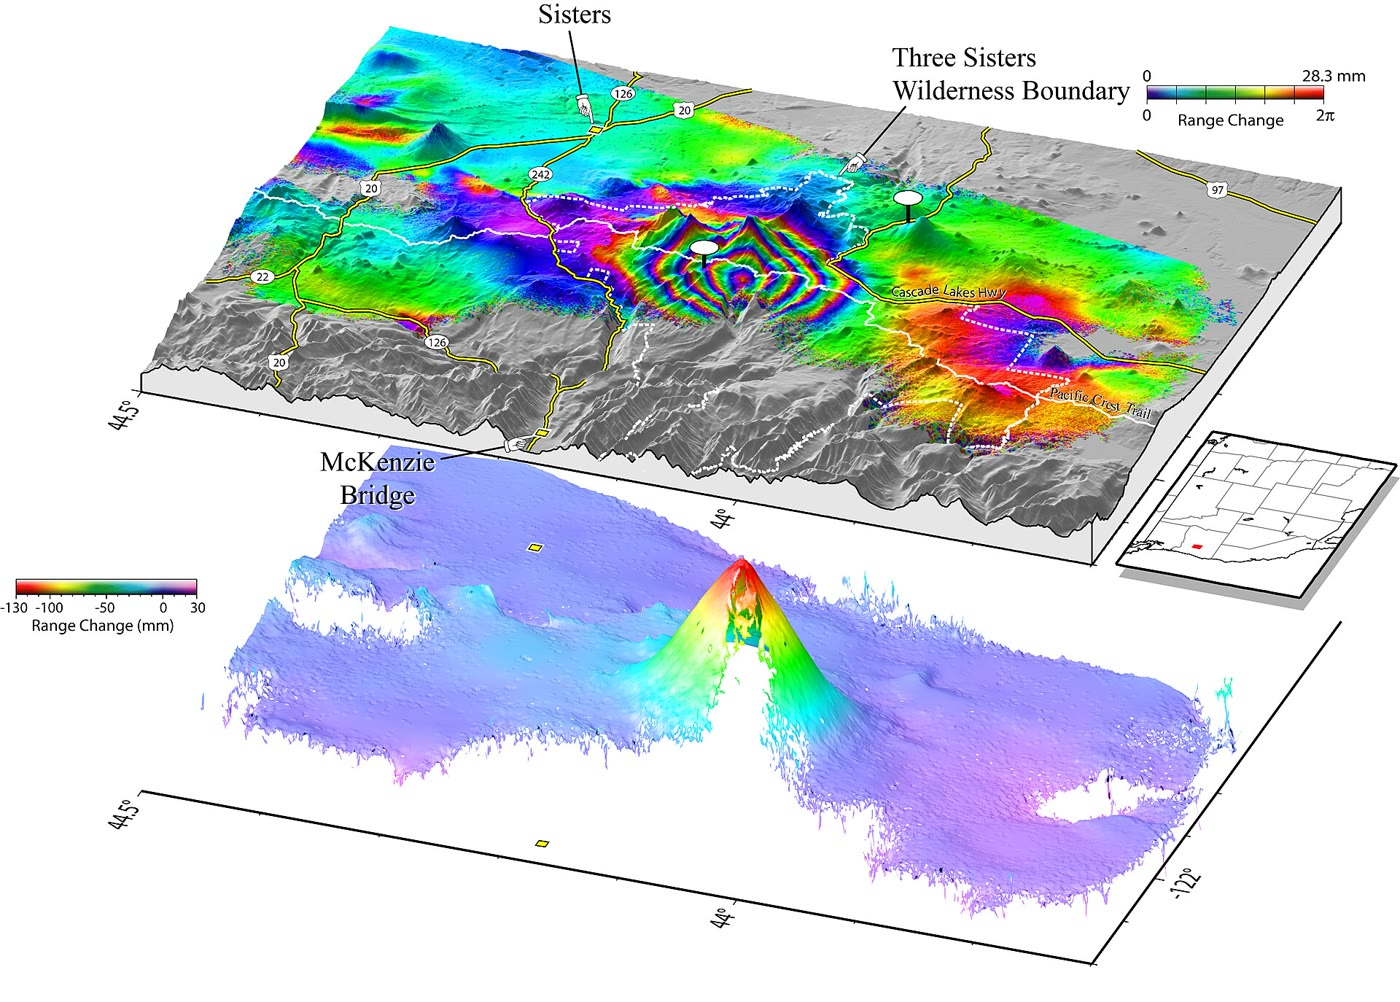
\includegraphics[width=0.86\linewidth]{images/book5/b3-three-sisters-insar.jpg}
\par\smallskip{\small ऊपर, ओरेगन के थ्री सिस्टर्स ज्वालामुखीय केंद्र का \omterm{def:b3:remote-sensing-gis:insar}{व्यतिकरण-लेख},
1995--2001 का, उच्चावच पर चढ़ाया हुआ: रंगों का हर चक्र
\qty{28.3}{mm} परास परिवर्तन है, और केंद्र पर छल्लों का बुल्स-आई
उत्थान दर्शाता है। नीचे, वही आँकड़े कला-अनावरित करके
उच्चावच के रूप में खींचे गए हैं: केंद्र पर परास अधिकतम \qty{130}{mm} घटती है। U.S.
Geological Survey (Wicks और अन्य, 2002), सार्वजनिक
डोमेन।}\label{fig:b3:remote-sensing-gis:three-sisters}
\end{omfigure}
% ledger: photo:b3-three-sisters-insar, usgs:insar-fs

\begin{inthelab}[भू-केंद्र]
\begin{minipage}[t]{0.55\linewidth}\vspace{0pt}
एक इमेजिंग उपग्रह, जब उस स्थान के ऊपर से गुज़रता है जिसका वह चित्र लेता है,
उससे कहीं अधिक अभिलेखित करता है जितना वह भेज सकता है। सेंटिनल-1 उपग्रह का रडार
हर कक्षा के अधिकतम आधे घंटे तक चित्र ले सकता है, और आँकड़े
उपग्रह पर संचित करता है, 1410 गीगाबिट तक; उन्हें दो चैनलों पर भेजता है,
प्रत्येक 260 मेगाबिट प्रति सेकंड की दर से, इसलिए पूरा भंडार ख़ाली होने में लगभग 45 मिनट लगते हैं।
एक भू-केंद्र इन्हें ग्रहण करता है: जब उपग्रह क्षितिज के ऊपर उठता है, तब डिश
उसकी ओर मुड़ती है, आकाश में उसका पीछा करती है और अस्त होते समय उसे छोड़ देती है,
जबकि संचालक जाँचते हैं कि आँकड़ों की धारा पूरी पहुँची है। आँकड़े फिर
एक संसाधन केंद्र को जाते हैं, जहाँ कच्ची प्रतिध्वनियाँ चित्र बन जाती हैं।
\end{minipage}\hfill
\begin{minipage}[t]{0.42\linewidth}\vspace{0pt}
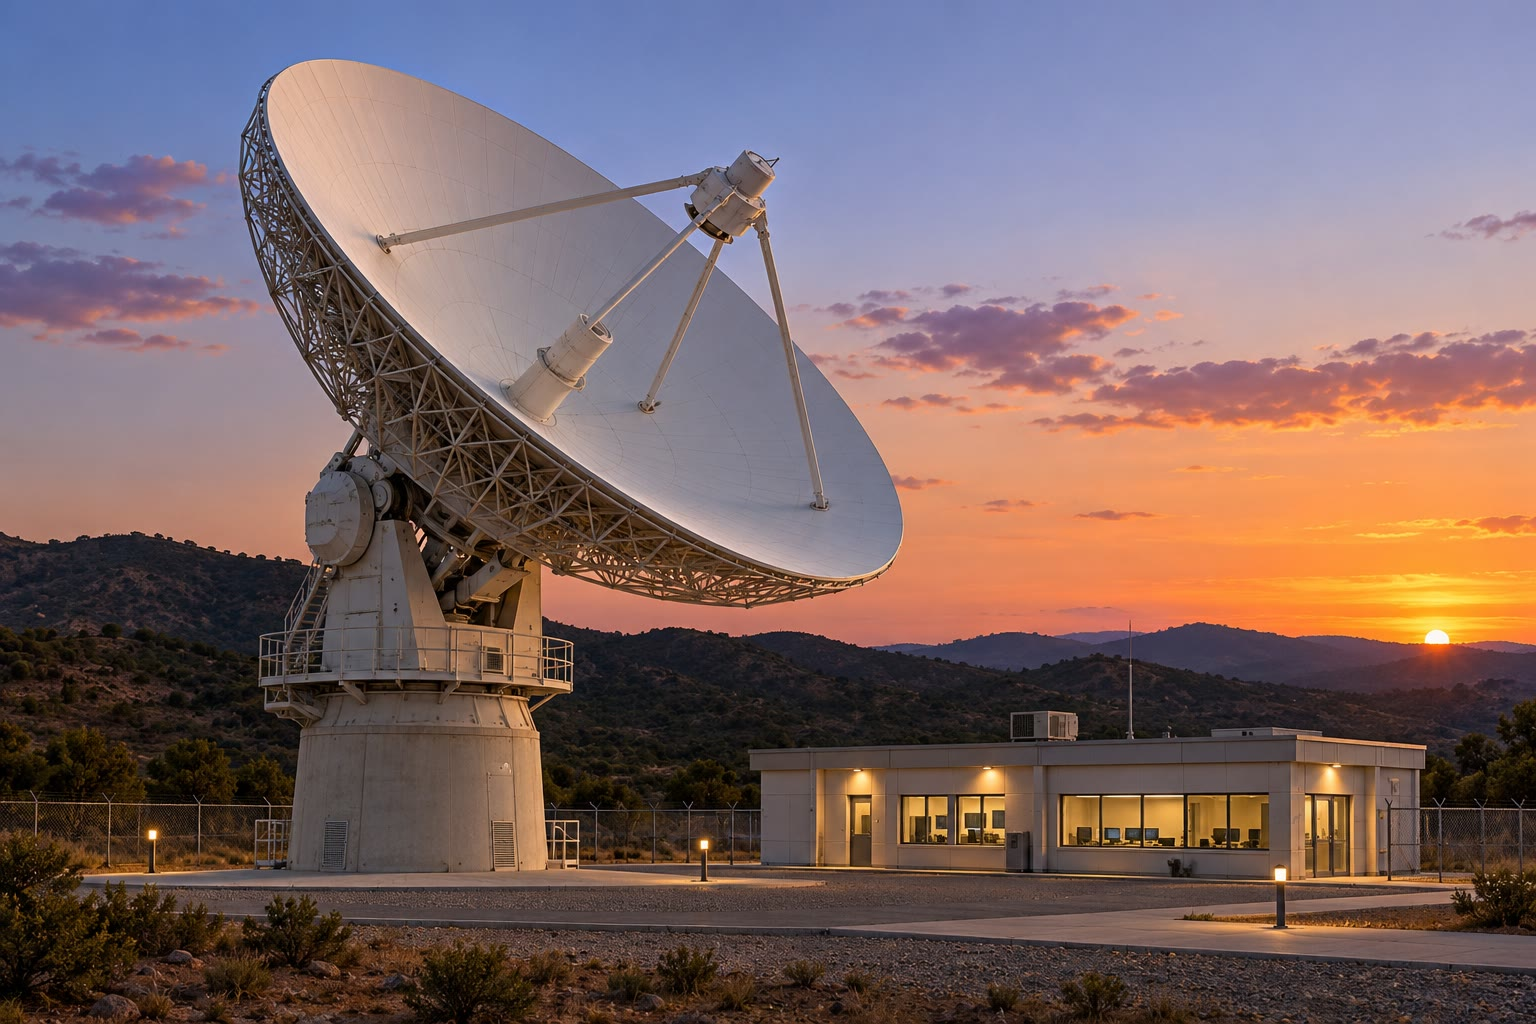
\includegraphics[width=\linewidth]{images/book5/ai/b3-ground-station.jpg}

{\scriptsize संध्या के समय एक उपग्रह भू-केंद्र: एक बड़ी ट्रैकिंग डिश और
उसका संचालन भवन (AI से बनाया गया चित्रण)।}
\end{minipage}
\end{inthelab}
% ledger: esa:s1-downlink

\section{भौगोलिक सूचना तंत्र}\label{sec:b3:remote-sensing-gis:gis}

उपग्रहों के चित्र, भूमि का अंकीय उन्नयन मॉडल, भूवैज्ञानिक
मानचित्र, कुएँ और सड़कें एक भौगोलिक
सूचना तंत्र की परतें हैं, जो उन्हें एक साझा निर्देशांक-ढाँचे में
संग्रहित करता है और उनके साथ परिकलन करता है।

\begin{definition}[रैस्टर आँकड़े और सदिश आँकड़े]\label{def:b3:remote-sensing-gis:data-models}
\emph{रैस्टर आँकड़े}\index{रैस्टर आँकड़े} एक परत को कोशिकाओं के एक जाल द्वारा
निरूपित करते हैं, जिनमें से हर कोशिका एक मान धारण करती है: परावर्तकता, उन्नयन या वर्ग।
\emph{सदिश आँकड़े}\index{सदिश आँकड़े (GIS)} उसे बिंदुओं, रेखाओं
और बहुभुजों द्वारा निरूपित करते हैं, जिनका स्थान उनके शीर्षों के निर्देशांकों से दिया जाता है, और
हर एक के साथ सारणी में विशेषताओं की एक पंक्ति जुड़ी होती है।
\end{definition}

\begin{omfigure}
\centering
\begin{tikzpicture}[x=0.5cm, y=0.5cm, font=\scriptsize]
\begin{scope}
\draw[black!40] (0,0) rectangle (10,7);
\fill[omSea!50, draw=omDef, thick] (3,4.5) ellipse (1.8 and 1.2);
\draw[omDef, very thick] (4.8,4.5) -- (7,3.5) -- (10,2);
\fill[red!70!black] (7,5.5) circle (0.14); \fill[red!70!black] (2,1.5) circle (0.14);
\node[anchor=south] at (5,7.1) {सदिश};
\node at (3,4.5) {झील};
\node[anchor=south west] at (7.1,5.6) {कुआँ 1};
\node[anchor=south west] at (2.1,1.6) {कुआँ 2};
\node[anchor=north east] at (9.9,2.2) {नदी};
\end{scope}
\begin{scope}[xshift=6.5cm]
\foreach \i/\j in {1/4,2/4,3/4,4/4,2/3,3/3,2/5,3/5} {\fill[omSea!50] (\i,\j) rectangle ++(1,1);}
\foreach \i/\j in {5/4,6/3,7/3,8/2,9/2} {\fill[omDef!70] (\i,\j) rectangle ++(1,1);}
\foreach \i/\j in {7/5,2/1} {\fill[red!70!black] (\i,\j) rectangle ++(1,1);}
\draw[black!30, step=1] (0,0) grid (10,7);
\draw[black!40] (0,0) rectangle (10,7);
\node[anchor=south] at (5,7.1) {रैस्टर};
\end{scope}
\end{tikzpicture}
\par\smallskip{\small वही मानचित्र सदिश आँकड़ों के रूप में (बाएँ: एक बहुभुज, एक रेखा
और दो बिंदु, जो स्थिति में सटीक हैं, हर एक अपनी विशेषताओं सहित) और \omterm{def:b3:remote-sensing-gis:data-models}{रैस्टर आँकड़ों} के रूप में
(दाएँ: हर कोशिका का एक मान, झील उन कोशिकाओं से जिनका केंद्र उसके भीतर है,
नदी और कुएँ उन कोशिकाओं से जिन्हें वे काटते हैं)। रैस्टर के साथ परिकलन कोशिका-दर-कोशिका सरल है;
सदिश परत किसी भी पैमाने पर आकृतियाँ और टोपोलॉजी
सुरक्षित रखती है।}\label{fig:b3:remote-sensing-gis:raster-vector}
\end{omfigure}

\begin{definition}[भू-संदर्भन]\label{def:b3:remote-sensing-gis:georef}
\emph{भू-संदर्भन}\index{भू-संदर्भन} वह है जिसमें किसी निर्धारित प्रक्षेपण के मानचित्र-निर्देशांक
किसी चित्र के हर पिक्सल और रेखाचित्र के हर शीर्ष को दिए जाते हैं,
ऐसे भू-नियंत्रण बिंदुओं पर एक रूपांतरण बैठाकर दिए जाते हैं,
जिनकी स्थितियाँ दोनों में ज्ञात हों।
\end{definition}

प्रक्षेपित ढाँचे में उत्तर-ऊपर रैस्टर के लिए रूपांतरण आफ़ाइन है:
स्तंभ $i$ और पंक्ति $j$ वाली कोशिका का कोना $E = E_0 + i\,\Delta$,
$N = N_0 - j\,\Delta$ पर होता है, जहाँ $\Delta$ कोशिका का आकार है। उपग्रह चित्र
पहले ऐसे ही एक जाल में पुनर्नमूनित किया जाता है; अलग-अलग प्रक्षेपणों की परतें
संयोजित करने से पहले एक में प्रक्षेपित की जाती हैं।

\begin{method}[अंकीय उन्नयन मॉडल से ढलान, पहलू और छायांकित उच्चावच]\label{met:b3:remote-sensing-gis:slope}
उन्नयनों $z_{i,j}$ के एक जाल पर, जिसका अंतराल $\Delta$ है ($i$ पूर्व की ओर, $j$
उत्तर की ओर), केंद्रीय अंतरों से प्रवणता का अनुमान लगाइए,
\[
\frac{\partial z}{\partial x} \approx \frac{z_{i+1,j} - z_{i-1,j}}{2\Delta} ,
\qquad
\frac{\partial z}{\partial y} \approx \frac{z_{i,j+1} - z_{i,j-1}}{2\Delta} .
\]
\emph{ढलान} $S = \arctan|\nabla z|$ है; \emph{पहलू} उस दिगंश को कहते हैं
जो सबसे तीव्र अवरोहण की दिशा है, यानी $-\nabla z$ की दिशा, $A =
\operatorname{atan2}(-\partial z/\partial x, -\partial z/\partial y)$
उत्तर से घड़ी की सुई की दिशा में मापा जाता है। \emph{छायांकित उच्चावच} के लिए
दिगंश $A_0$ से आने वाले और खमध्य-कोण $Z$ पर स्थित प्रकाश के लिए $\cos Z\cos S + \sin Z\sin S
\cos(A_0 - A)$ है, जो प्रकाश और भूमि के अभिलंब के बीच के कोण की कोज्या है,
जहाँ यह ऋणात्मक हो वहाँ शून्य रखा जाता है।
\end{method}

समतल के लिए केंद्रीय अंतर सटीक है, और अन्यथा इसकी त्रुटि
$\Delta^2 z'''/6$ होती है; पुस्तक 3 (स्नातक वर्ष 1) में वार्डन पहाड़ियों का
छायांकित उच्चावच इसी विधि से परिकलित किया गया था, उत्तर-पश्चिम से प्रकाशित करके।
अवकलज जाल की त्रुटियों को बढ़ाते हैं: जिस मॉडल की पंक्तियों के बीच चरण हों,
उसके ढलान-मानचित्र में वे धारियों के रूप में दिखती हैं।

\begin{definition}[मानचित्र बीजगणित]\label{def:b3:remote-sensing-gis:map-algebra}
\emph{मानचित्र बीजगणित}\index{मानचित्र बीजगणित} वह संक्रिया है जिसमें एक नई रैस्टर परत
कोशिका-दर-कोशिका, उसी जाल की एक या अधिक परतों से परिकलित की जाती है:
अंकगणित द्वारा (दो बैंडों से NDVI), तुलना द्वारा (वे कोशिकाएँ जो
\ang{15} से अधिक ढालू हैं), तार्किक संक्रियाओं द्वारा (और, या, नहीं), या
कोशिका के पड़ोस से (ढलान)।
\end{definition}

\begin{definition}[बफ़र; अध्यारोपण]\label{def:b3:remote-sensing-gis:operations}
किसी लक्षण से दूरी $d$ पर \emph{बफ़र}\index{बफ़र (GIS)} मानचित्र का वह भाग
है जो उससे $d$ की दूरी के भीतर आता है। एक
\emph{अध्यारोपण}\index{अध्यारोपण (GIS)} एक ही क्षेत्र की दो या अधिक परतों को एक में जोड़ता है,
जिसमें परिणाम के हर स्थान पर उन सबकी विशेषताएँ
एक साथ रहती हैं; एक साथ कई शर्तों को पूरा करने वाले स्थानों का चयन
सबसे सामान्य उपयोग है।
\end{definition}

\begin{omfigure}
\centering
\begin{tikzpicture}
\begin{groupplot}[group style={group size=2 by 2, horizontal sep=2.0cm, vertical sep=1.5cm},
  width=0.43\linewidth, axis equal image, enlargelimits=false,
  xmin=0, xmax=10, ymin=0, ymax=8,
  tick label style={font=\scriptsize}, label style={font=\small}, title style={font=\small}]
\nextgroupplot[title={(क) ढलान (अंश)}, ylabel={उत्तर (km)}, colormap/viridis,
  point meta min=0, point meta max=24, colorbar right,
  colorbar style={width=0.18cm, ytick={0,5,10,15,20}, tick label style={font=\tiny}, axis equal=false}]
\addplot[matrix plot*, mesh/cols=101, point meta=explicit] table[x=x, y=y, meta=slope] {figdata/out/bachelor-3-varden_gis-grid.dat};
\addplot[white, thick] table {figdata/out/shared-region-river.dat};
\nextgroupplot[title={(ख) पहलू},
  colormap={aspect}{rgb255=(220,20,30) rgb255=(240,200,0) rgb255=(30,170,60) rgb255=(30,90,220) rgb255=(220,20,30)},
  point meta min=0, point meta max=360, colorbar right,
  colorbar style={width=0.18cm, ytick={0,90,180,270,360}, yticklabels={\omnameCompassN,\omnameCompassE,\omnameCompassS,\omnameCompassW,\omnameCompassN}, tick label style={font=\tiny}, axis equal=false}]
\addplot[matrix plot*, mesh/cols=101, point meta=explicit] table[x=x, y=y, meta=aspect] {figdata/out/bachelor-3-varden_gis-grid.dat};
\addplot[black, thick] table {figdata/out/shared-region-river.dat};
\nextgroupplot[title={(ग) दो परतें}, xlabel={पूर्व (km)}, ylabel={उत्तर (km)},
  colormap={lay}{rgb255=(245,245,245) rgb255=(150,150,150) rgb255=(225,195,140) rgb255=(120,70,20)},
  colormap access=piecewise constant, point meta min=-0.5, point meta max=3.5,
  legend columns=2, legend style={font=\tiny, at={(0.5,-0.3)}, anchor=north, /tikz/every even column/.append style={column sep=4pt}}]
\addplot[matrix plot*, mesh/cols=101, point meta=explicit, forget plot] table[x=x, y=y, meta=layers] {figdata/out/bachelor-3-varden_gis-grid.dat};
\addplot[omDef, thick, forget plot] table {figdata/out/shared-region-river.dat};
\addlegendimage{area legend, fill={rgb,255:red,150;green,150;blue,150}, draw=black!40}
\addlegendentry{\ang{15} से अधिक ढालू}
\addlegendimage{area legend, fill={rgb,255:red,225;green,195;blue,140}, draw=black!40}
\addlegendentry{शेल}
\addlegendimage{area legend, fill={rgb,255:red,120;green,70;blue,20}, draw=black!40}
\addlegendentry{दोनों}
\nextgroupplot[title={(घ) अध्यारोपण}, xlabel={पूर्व (km)},
  colormap={cls}{rgb255=(245,245,245) rgb255=(225,195,140) rgb255=(190,150,90) rgb255=(200,20,30)},
  colormap access=piecewise constant, point meta min=-0.5, point meta max=3.5,
  legend columns=2, legend style={font=\tiny, at={(0.5,-0.3)}, anchor=north, /tikz/every even column/.append style={column sep=4pt}}]
\addplot[matrix plot*, mesh/cols=101, point meta=explicit, forget plot] table[x=x, y=y, meta=class] {figdata/out/bachelor-3-varden_gis-grid.dat};
\addplot[omDef, thick, forget plot] table {figdata/out/shared-region-river.dat};
\addplot[black, thin, dashed, unbounded coords=jump] table[x=x, y=y] {figdata/out/bachelor-3-varden_gis-buffer.dat};
\addlegendentry{\qty{1}{km} बफ़र}
\addlegendimage{area legend, fill={rgb,255:red,225;green,195;blue,140}, draw=black!40}
\addlegendentry{शेल}
\addlegendimage{area legend, fill={rgb,255:red,190;green,150;blue,90}, draw=black!40}
\addlegendentry{बफ़र में शेल}
\addlegendimage{area legend, fill={rgb,255:red,200;green,20;blue,30}, draw=black!40}
\addlegendentry{चयनित}
\end{groupplot}
\end{tikzpicture}
\par\smallskip{\small वार्डन पहाड़ियों पर एक GIS सत्र, उनके अंकीय उन्नयन मॉडल से,
जो \qty{100}{m} के जाल पर है। (क)~ढलान, घाटी की ढलानों पर \ang{23} तक;
(ख)~पहलू, यानी वह दिशा जिधर भूमि मुख करती है, नदी के दोनों किनारे
एक-दूसरे की ओर मुख किए हैं; (ग)~दो परतें, वे कोशिकाएँ जो \ang{15} से अधिक ढालू हैं
और जुरासिक शेल का अनावरण; (घ)~उनका \omterm{def:b3:remote-sensing-gis:operations}{अध्यारोपण}
नदी के \qty{1}{km} \omterm{def:b3:remote-sensing-gis:operations}{बफ़र} (धराशायी) के साथ उसका \omterm{def:b3:remote-sensing-gis:operations}{अध्यारोपण}: नदी के ऊपर का
\qty{0.32}{km^2} ढालू शेल, जो भूमि के उस भाग की प्रारंभिक छानबीन है जो खिसक
सकता है।}\label{fig:b3:remote-sensing-gis:varden}
\end{omfigure}

ऊपर का चित्र पूरी शृंखला दिखाता है: उन्नयन ग्रिड पर \omterm{def:b3:remote-sensing-gis:map-algebra}{मानचित्र बीजगणित}
ढलान और ढलान-दिशा देता है; एक तुलना ढलान को एक परत में बदल देती है,
जिसमें तीव्र कोशिकाएँ हैं; भूवैज्ञानिक मानचित्र शेल देता है; नदी का
\omterm{def:b3:remote-sensing-gis:operations}{बफ़र} तीसरी परत देता है; उनका प्रतिच्छेद, तार्किक
\emph{और} के साथ \omterm{def:b3:remote-sensing-gis:operations}{अध्यारोपण}, 8181 में से 32 कोशिकाएँ छोड़ता है। उत्तर उतना ही अच्छा है, जितनी
अच्छी ये परतें हैं; मोटे ग्रिड पर ढलान कम तीव्र निकलते हैं और कम कोशिकाएँ पास होती हैं।

\begin{definition}[पर्यवेक्षित वर्गीकरण; भ्रम आव्यूह]\label{def:b3:remote-sensing-gis:classification}
\emph{पर्यवेक्षित वर्गीकरण}\index{पर्यवेक्षित वर्गीकरण} किसी छवि के प्रत्येक पिक्सल को
वर्गों के एक समुच्चय में से किसी एक में रखता है, उन नियमों या सांख्यिकी के आधार पर
जो उन प्रशिक्षण पिक्सलों से सीखे गए हैं जिनका वर्ग भूमि पर ज्ञात है।
इसका \emph{भ्रम आव्यूह}\index{भ्रम आव्यूह} एक अलग
संदर्भ पिक्सलों के समुच्चय के लिए गिनता है कि प्रत्येक वास्तविक वर्ग के कितने
पिक्सल किस वर्ग को सौंपे गए: $n_{ij}$ पिक्सल जिन्हें $i$ के रूप में वर्गीकृत किया गया, वास्तव में $j$ के हैं।
\end{definition}

विकर्ण पर वे पिक्सल आते हैं जिनका वर्गीकरण सही हुआ। $N$ संदर्भ पिक्सलों के साथ,
\emph{समग्र यथार्थता} $\sum_i n_{ii}/N$ है। किसी वर्ग की \emph{उपयोगकर्ता
यथार्थता}, पंक्ति योग पर $n_{ii}$, वह संभाविता है कि
एक पिक्सल, जिसे मानचित्र $i$ कहता है, $i$ ही है; इसकी \emph{उत्पादक
यथार्थता}, स्तंभ योग पर $n_{ii}$, यह संभाविता है कि एक वास्तविक $i$ को $i$ के रूप में मानचित्रित किया गया।
\emph{कप्पा} गुणांक समग्र यथार्थता $p_o$ की तुलना
उस यथार्थता $p_e = \sum_i (\text{पंक्ति}_i)(\text{स्तंभ}_i)/N^2$ से करता है, जो समान योगों के साथ यादृच्छिक असाइनमेंट से प्राप्त होती
है: $\kappa = (p_o - p_e)/(1 -
p_e)$।

\begin{center}
\small
\begin{tabular}{l|ccc|c}
\hline
वर्गीकृत \textbackslash{} संदर्भ & जल & वन & नंगी चट्टान & योग \\
\hline
जल & 45 & 2 & 0 & 47 \\
वन & 3 & 38 & 7 & 48 \\
नंगी चट्टान & 0 & 5 & 30 & 35 \\
\hline
योग & 48 & 45 & 37 & 130 \\
\hline
\end{tabular}
\end{center}

इस काल्पनिक उदाहरण में, 130 में से 113 पिक्सल सही हैं, समग्र
यथार्थता \qty{86.9}{\percent} है। वन की उपयोगकर्ता यथार्थता
$38/48 = \qty{79}{\percent}$ है, परंतु उत्पादक यथार्थता $38/45 =
\qty{84}{\percent}$ है: नंगी चट्टान के सात पिक्सल, शायद छाया में, वन
कहे गए। यादृच्छिक असाइनमेंट से $p_e = 0.338$ प्राप्त होता, और $\kappa =
0.80$।

\section{अभ्यास}

\begin{exercise}[$\star$]\label{exo:b3:remote-sensing-gis:1}
किसी इमेजर के लाल बैंड में एक क्षेत्र की परावर्तकता 0.06 है और
निकट-अवरक्त बैंड में 0.42 है; इसके बगल में एक जुती हुई भूमि की परावर्तकता क्रमशः 0.21 और
0.28 है। दोनों का NDVI परिकलित कीजिए और बताइए कि प्रत्येक मान क्या संकेत देता है।
\end{exercise}

\begin{exercise}[$\star$]\label{exo:b3:remote-sensing-gis:2}
लैंडसैट~8 इमेजर \qty{185}{km} चौड़ी पट्टी को ढकता है, जिसके पिक्सल
\qty{30}{m} के हैं, और इसका पैन-क्रोमैटिक बैंड \qty{15}{m} पिक्सलों वाला है। (क)~कितने
पिक्सल पट्टी की एक रेखा में प्रत्येक स्थिति में होते हैं? (ख)~कितने स्तर
12 बिट और 8 बिट देते हैं? (ग)~लैंडसैट~8 का
अकेले \omterm{def:b3:remote-sensing-gis:resolutions}{पुनरागमन काल}, और लैंडसैट 8 व 9 साथ मिलकर का, क्या है?
\end{exercise}

\begin{exercise}[$\star$]\label{exo:b3:remote-sensing-gis:3}
(क)~एक अवधसान करती द्रोणी के सेंटिनल-1 \omterm{def:b3:remote-sensing-gis:insar}{व्यतिकरण-लेख} ($\lambda = \qty{5.55}{cm}$) पर
छह फ्रिंज स्थिर किनारे को केंद्र से अलग करते हैं।
केंद्र पर \omterm{def:b3:remote-sensing-gis:insar}{दृष्टि-रेखा} का परिवर्तन क्या है? (ख)~एक फ्रिंज का मान
\qty{5.66}{cm} तरंगदैर्घ्य वाले एक पुराने उपग्रह के लिए क्या होगा?
\end{exercise}

\begin{exercise}[$\star$]\label{exo:b3:remote-sensing-gis:4}
एक लेज़र ऊँचाईमापी भूमि से \qty{500}{km} ऊपर है। (क)~एक स्पंद को
लौटने में कितना समय लगता है? (ख)~यदि प्रत्येक फ़ोटॉन का समय \qty{800}{ps} तक मापा जाए, तो
एक परास कितनी सटीक होगी?
\end{exercise}

\begin{exercise}[$\star\star$]\label{exo:b3:remote-sensing-gis:5}
लैंडसैट~8 के बैंड~10 का एक पिक्सल लीजिए ($\lambda = \qty{10.9}{\micro\metre}$),
जिसका \omterm{def:b3:remote-sensing-gis:atm-correction}{वायुमंडलीय संशोधन} के बाद स्पेक्ट्रमी विकिरण
\qty{9.0}{W.m^{-2}.sr^{-1}.\micro\metre^{-1}} है। (क)~इसका \omterm{def:b3:remote-sensing-gis:brightness}{दीप्ति
तापमान} परिकलित कीजिए। (ख)~सतह एक घास का मैदान है, जिसकी उत्सर्जकता 0.98 है: इसका
गतिज तापमान क्या है?
\end{exercise}

\begin{exercise}[$\star\star$]\label{exo:b3:remote-sensing-gis:6}
सेंटिनल-1 रडार \qty{693}{km} ऊपर उड़ता है, और इसका एंटीना \qty{12.3}{m}
लंबा है, $\lambda = \qty{5.55}{cm}$ पर। (क)~पृथ्वी की वक्रता की उपेक्षा करते हुए
एक ऐसे बिंदु तक की तिर्यक परास परिकलित कीजिए जो
\ang{35} के आपतन-कोण पर दिखता है। (ख)~उस लंबाई के एक वास्तविक एंटीना से वहाँ
कौन-सा दिगंश विभेदन मिलेगा, और संश्लेषित द्वारक क्या देता है? (ग)~संश्लेषित द्वारक
की लंबाई कितनी है?
\end{exercise}

\begin{exercise}[$\star\star$]\label{exo:b3:remote-sensing-gis:7}
\qty{30}{m} कोशिकाओं वाले अंकीय उन्नयन मॉडल की एक $3\times3$ खिड़की
उत्तर को ऊपर रखकर इसमें ये मान पढ़े जाते हैं,
\[
\begin{matrix} 412 & 418 & 425 \\ 405 & 410 & 418 \\ 398 & 401 & 409 \end{matrix}
\qquad (\unit{m}).
\]
केंद्र कोशिका पर केंद्रीय अंतरों द्वारा प्रवणता, ढलान-दिशा
और उत्तर-पश्चिम से आते प्रकाश के लिए छायांकन, जो
क्षितिज से \ang{45} ऊपर है, परिकलित कीजिए।
\end{exercise}

\begin{exercise}[$\star\star$]\label{exo:b3:remote-sensing-gis:8}
एक भू-आवरण मानचित्र की 160 संदर्भ पिक्सलों से जाँच की गई है (पंक्तियाँ: मानचित्र;
स्तंभ: वास्तविकता; वर्ग जल, वन, फ़सलें, नगर):
\[
\begin{pmatrix} 48 & 3 & 1 & 0 \\ 4 & 37 & 6 & 1 \\ 2 & 5 & 29 & 2 \\ 0 & 1 & 2 & 19 \end{pmatrix} .
\]
समग्र यथार्थता परिकलित कीजिए, और प्रत्येक वर्ग की उपयोगकर्ता व उत्पादक यथार्थताएँ,
तथा कप्पा। कौन-सा वर्ग सबसे अधिक बार चूकता है?
\end{exercise}

\begin{exercise}[$\star\star$]\label{exo:b3:remote-sensing-gis:9}
\qty{100}{m} का एक तापीय पिक्सल, जिसमें \qty{1443}{K} पर एक ताज़ा लावा-प्रवाह है,
जो उसके \qty{4}{\percent} भाग को ढकता है; शेष भूतल \qty{290}{K} पर है; दोनों को
कृष्ण पिंड मानिए। (क)~पिक्सल का
\qty{10.9}{\micro\metre} पर \omterm{def:b3:remote-sensing-gis:brightness}{दीप्ति तापमान} परिकलित कीजिए और उसकी तुलना माध्य तापमान से कीजिए।
(ख)~लावा और भूतल की कृष्ण-पिंड विकिरणता का अनुपात परिकलित कीजिए,
\qty{2.2}{\micro\metre} पर, तथा वहाँ पिक्सल का \omterm{def:b3:remote-sensing-gis:brightness}{दीप्ति तापमान} भी
परिकलित कीजिए। कौन-सा बैंड लावा को बेहतर पहचानता है?
\end{exercise}

\begin{exercise}[$\star\star\star$]\label{exo:b3:remote-sensing-gis:10}
एक ही विरूपण के दो \omterm{def:b3:remote-sensing-gis:insar}{व्यतिकरण-लेख} दो पासों से बने हैं, एक में उपग्रह भूमि के पूर्व में
और दूसरे में पश्चिम में, दोनों
\ang{35} आपतन-कोण पर। एक बिंदु पर \omterm{def:b3:remote-sensing-gis:insar}{दृष्टि-रेखा} पहले में
\qty{64}{mm} और दूसरे में \qty{38}{mm} घटती है।
उत्तर--दक्षिण गति न मानकर, ऊर्ध्वाधर तथा
पूर्व की ओर के विस्थापन परिकलित कीजिए। एक पास पर्याप्त क्यों नहीं है?
\end{exercise}

\begin{exercise}[$\star\star\star$]\label{exo:b3:remote-sensing-gis:11}
\omterm{def:b3:remote-sensing-gis:insar}{कला अनावरण} वहाँ विफल होता है जहाँ पड़ोसी पिक्सलों के बीच कला $\pi$ से
अधिक छलाँग लगाती है। (क)~दिखाइए कि एक पिक्सल से अगले तक \omterm{def:b3:remote-sensing-gis:insar}{दृष्टि-रेखा}
$\lambda/4$ से कम बदलनी चाहिए, जो सेंटिनेल-1 के लिए \qty{13.9}{mm} है।
(ख)~एक मोगी स्रोत के लिए, जो $z_0 = \qty{4}{km}$ गहराई पर है, जिसमें $\Delta V =
\qty{e7}{m^3}$ और $\nu = 0.25$ है, ऊर्ध्वाधर दिशा से देखने पर, दिखाइए कि $u_z$ की
सबसे तीव्र प्रवणता $r = z_0/2$ पर है, और उसे परिकलित कीजिए। (ग)~वह सबसे बड़ा
पिक्सल आकार क्या है जो पट्टियों को विभेदनीय रखता है?
\end{exercise}

\begin{exercise}[$\star\star\star$]\label{exo:b3:remote-sensing-gis:12}
(क)~दिखाइए कि अऋणात्मक परावर्तकताओं के लिए NDVI $-1$ और $+1$ के बीच होता है,
और यह कि जब दोनों परावर्तकताओं को एक ही गुणक से गुणा किया जाता है, तो यह अपरिवर्तित रहता है।
(ख)~घास की परावर्तकताएँ लाल बैंड में 0.051 और
निकट-अवरक्त बैंड में 0.502 हैं। एक असंशोधित प्रतिबिंब में पथ-विकिरणता जुड़ जाती है
जो लाल में 0.03 और निकट-अवरक्त में 0.01 के तुल्य है। इसके साथ और इसके बिना
NDVI परिकलित कीजिए। (ग)~धुंधले दिन पर असंशोधित प्रतिबिंबों से बने NDVI
के मानचित्र के लिए इससे क्या तात्पर्य निकलता है?
\end{exercise}

\section{समस्या: माउंट हैल्व्रेन पर एक उभरता पार्श्व}

\begin{problem}[{सप्ताहांत समस्या --- वनस्पति, ऊष्मा और एक काल्पनिक ज्वालामुखी पर रडार
व्यतिकरण-लेख}]
\label{pb:b3:remote-sensing-gis:1}
माउंट हैल्व्रेन, एक काल्पनिक ज्वालामुखी, ने 1890, 1960
और 2005 में अपने वनाच्छादित पार्श्वों पर लावा-प्रवाह उगले हैं। इसके शिखर पर
एक फ़्यूमरोल क्षेत्र भाप छोड़ता है। एक हाल के वर्ष के उपग्रह आँकड़े नीचे दिए गए हैं।

\medskip\noindent\textbf{भाग I --- लावा-प्रवाहों पर वनस्पति।} संशोधित
परावर्तकताएँ लाल और निकट-अवरक्त बैंडों में:
\begin{center}
\small
\begin{tabular}{lcccc}
\hline
सतह & वन & 1890 का प्रवाह & 1960 का प्रवाह & 2005 का प्रवाह \\
\hline
लाल & 0.04 & 0.07 & 0.11 & 0.12 \\
निकट-अवरक्त & 0.38 & 0.30 & 0.21 & 0.14 \\
\hline
\end{tabular}
\end{center}
\begin{enumerate}
\item चारों सतहों का NDVI परिकलित कीजिए।
\item प्रवाहों को उनकी वनस्पति की पुनर्प्राप्ति के आधार पर क्रम दीजिए। क्या यह क्रम
  उनकी आयु के क्रम जैसा है?
\item 2005 के प्रवाह का NDVI शून्य क्यों नहीं है, यद्यपि उस पर
  लगभग कुछ नहीं उगता?
\item तीव्र ढालों वाले और असमान रूप से प्रकाशित ज्वालामुखी-पार्श्वों पर, NDVI
  निकट-अवरक्त परावर्तकता अकेले की तुलना में क्यों अधिक विश्वसनीय है?
\end{enumerate}

\medskip\noindent\textbf{भाग II --- फ़्यूमरोल क्षेत्र।} तापीय
बैंड में ($\lambda = \qty{10.9}{\micro\metre}$ मानिए) संशोधित विकिरणता
फ़्यूमरोल से दूर शिखर पठार के एक \qty{100}{m} पिक्सल की
\qty{8.40}{W.m^{-2}.sr^{-1}.\micro\metre^{-1}} है, और फ़्यूमरोल-क्षेत्र वाले पिक्सल की
विकिरणता \qty{9.95}{W.m^{-2}.sr^{-1}.\micro\metre^{-1}} है।
\begin{enumerate}[resume]
\item दोनों पिक्सलों के \omterm{def:b3:remote-sensing-gis:brightness}{दीप्ति तापमान} परिकलित कीजिए।
\item पठार की चट्टान की उत्सर्जकता 0.97 है। इसका गतिज
  तापमान क्या है?
\item फ़्यूमरोल के छिद्र और उनके चारों ओर की गर्म भूमि
  \qty{370}{K} पर हैं। उन्हें और पिक्सल के शेष भाग को कृष्ण पिंड मानते हुए,
  शेष भाग पठार की विकिरणता पर है, पिक्सल का कितना अंश वे ढकते हैं
  और कितना क्षेत्रफल?
\item पिक्सल का क्षेत्रफल-भारित माध्य तापमान उसके \omterm{def:b3:remote-sensing-gis:brightness}{दीप्ति तापमान} से क्यों
  कम रहता है?
\end{enumerate}

\medskip\noindent\textbf{भाग III --- व्यतिकरण-लेख।} सेंटिनेल-1 के दो
प्रतिबिंब ($\lambda = \qty{5.55}{cm}$, आपतन-कोण \ang{35}, उपग्रह पूर्व में)
48 दिन के अंतर पर लिए गए, पूर्वी ढाल पर एक बुल्स-आई दिखाते हैं।
एक स्थिर क्षेत्र से पैटर्न के केंद्र तक पाँच पूरी पट्टियाँ और
छठी पट्टी का चार-दसवाँ भाग गिना जाता है, और ये सभी उपग्रह की ओर की
गति के अर्थ में हैं।
\begin{enumerate}[resume]
\item दो प्रतिबिंब लगभग एक ही स्थिति से क्यों लिए जाने चाहिए, और एक ही
  उपग्रह के कितने कक्षीय चक्र उन्हें अलग करते हैं?
\item केंद्र पर \omterm{def:b3:remote-sensing-gis:insar}{दृष्टि-रेखा} के परिवर्तन को परिकलित कीजिए।
\item केंद्र पर भूमि केवल ऊर्ध्वाधर गति करती है। वहाँ का उत्थान
  परिकलित कीजिए।
\item समझाइए कि पैटर्न वृत्ताकार क्यों नहीं है, और किस ओर, पूर्व या
  पश्चिम, पट्टियाँ सघन हैं।
\item केंद्र से होकर उत्तर--दक्षिण रेखा के अनुदिश \omterm{def:b3:remote-sensing-gis:insar}{दृष्टि-रेखा} का परिवर्तन
  केंद्र से \qty{3.4}{km} दूरी पर अपने केंद्रीय मान के आधे तक गिर जाता है।
  इस रेखा का उपयोग क्यों किया जाता है, और एक मोगी
  स्रोत के लिए यह कौन-सी गहराई देती है?
\item केंद्र को उस अर्ध-ऊँचाई बिंदु से कितनी पट्टियाँ अलग करती हैं?
\item वायु में जलवाष्प दोनों तिथियों पर रडार तरंगों को भिन्न रूप से
  विलंबित कर सकता है और अपनी पट्टियाँ खींच सकता है। किसी अन्य तिथि-युग्म का
  दूसरा \omterm{def:b3:remote-sensing-gis:insar}{व्यतिकरण-लेख} दोनों को अलग पहचानने में कैसे सहायक होगा?
\end{enumerate}

\medskip\noindent\textbf{भाग IV --- आयतन।} $\nu = 0.25$ मानिए।
\begin{enumerate}[resume]
\item $u_z(0) = (1 - \nu)\Delta V/(\pi z_0^2)$ से स्रोत के आयतन का
  परिवर्तन परिकलित कीजिए।
\item इसे 48 दिन की अवधि में प्रति दिन और प्रति वर्ष के औसत दर के रूप में व्यक्त कीजिए।
\item सबसे बड़ा क्षैतिज विस्थापन परिकलित कीजिए, और वह कहाँ होता है।
\item यदि जलाशय त्रिज्या $z_0/3$ का एक गोला होता, तो उसका
  आयतन कितना होता, और परिवर्तन उसका कितना अंश निरूपित करता है?
\item त्रिज्या $z_0/3$ के गोले का परिमित आकार उत्थान को
  लगभग \qty{3}{\percent} बदल देता है। क्या यह प्रश्न~16 के उत्तर को
  उल्लेखनीय रूप से बदलता है, पट्टी-गणना की परिशुद्धता को देखते हुए?
\item भाग I और II से, या भूमि से कौन-सा अन्य प्रेक्षण
  भरते हुए जलाशय की व्याख्या का समर्थन करेगा?
\item माउंट हैल्व्रेन के नीचे के जलाशय का आयतन-परिवर्तन दस लाख घन मीटर में,
  दो सार्थक अंकों तक दीजिए।
\end{enumerate}
\end{problem}
% ledger: nasa:ndvi, esa:s1-sar, esa:s1-orbit, esa:s1-iw, dmodels:mogi, dmodels:mogi-radial, const:h, const:c, const:kB
